\chapter{Closing the Loop: Real Ensemble Training and Full Re-Validation}
\label{ch:closing}

Chapter~\ref{ch:integrity} closed on two explicitly unresolved items,
repeated in Section~\ref{sec:future}: whether the trained/random gap in
Table~\ref{tab:lhr_arms} survives a paired per-image test, and whether
ensemble guidance --- shown in that chapter only on no-policy,
generation-only arms --- actually closes the held-out transfer gap of
Table~\ref{tab:heldout} when a policy is \emph{trained under it} rather
than merely evaluated through it. This short chapter closes both, in a
later work session after the chapters above were written.

\section{Making Ensemble Guidance the Trained Default}

Ensemble guidance had remained disabled by default for comparability with
an earlier archived policy, meaning every trained-policy result in
Chapters~\ref{ch:results}--\ref{ch:integrity} --- including
Table~\ref{tab:heldout} and the trained arm of Table~\ref{tab:lhr_arms} ---
was produced under single-classifier guidance, even though
Section~\ref{sec:arm_results} had already shown ensemble guidance to be
the one countermeasure that helps. This was corrected: ensemble guidance
is now the default, with the previous behaviour still reachable if a
direct comparison to it is needed again.

Flipping a default is not, by itself, evidence of anything --- the trained
policies already on disk still reflected the old setting until retrained.
Two precautions were taken before that retraining could be trusted.
First, the training loop resumes from its last saved state and, on
finding the target number of episodes already reached, exits without
training a single new step while still re-saving its checkpoint files ---
a behaviour a preliminary test run confirmed directly, by loading the new
ensemble classifier correctly while silently re-stamping a policy that had
in fact finished training two days earlier under the old configuration.
Left unnoticed, this would have looked, from the output alone, like a
successful ensemble-guided training run. The previous checkpoints were
therefore archived rather than overwritten before any real retraining was
submitted, and a repeat of the same preliminary test then confirmed a
genuinely fresh run, with no prior state found to resume from. Second, the
evaluation pipeline writes its counterfactuals to the same directory every
comparison in earlier chapters depends on unless told otherwise; the new
run was tagged and routed to a separate location so that regenerating it
could not silently overwrite the results those comparisons still need.

With the prior checkpoints safely out of the way, both directional
policies were retrained from scratch under ensemble guidance: 800 episodes
each, confirmed by the training log showing the ensemble classifier
correctly loaded and no indication of resuming a previous run in either
direction.

\section{What Changed on the Guidance-Side Metrics}

Re-evaluating the freshly trained policies gives a mixed picture on the
metrics computed \emph{with} the guidance model, which is expected:
Section~\ref{sec:heldout} already established these cannot be trusted as
evidence of transfer, and ensemble validity --- asking two classifiers to
agree --- is a strictly harder bar than asking one.

\begin{itemize}[leftmargin=*]
  \item \textbf{Counterfactual Validity fell}, from mean $0.965$
        (single-classifier, Table~\ref{tab:results}) to mean $0.8375$
        (\ntop{} $=0.960$, \pton{} $=0.715$) --- consistent with a harder
        joint criterion, not a weaker policy.
  \item \textbf{Lesion Hit Rate rose}, to a $2.67\times$ lift over the
        radiologist-box chance baseline ($t=24.19$, $p=4.2\times10^{-53}$,
        $n=148$), above the single-classifier trained arm's $2.293\times$
        in Table~\ref{tab:lhr_arms}. Unlike Counterfactual Validity, LHR is
        scored against ground truth, not against any classifier, so this
        is a real (if not yet significance-tested against the old arm)
        improvement in \emph{where} the edit lands.
  \item \textbf{Edit concentration stayed diffuse}: $0.253$ (\ntop{}) and
        $0.318$ (\pton{}) against the $0.05$ uniform baseline --- close to
        the values in Section~\ref{sec:heldout} and still far short of the
        $\sim\!0.5$ that would indicate a focal, lesion-shaped edit.
\end{itemize}

None of this answers the actual question. It motivates re-running the one
check that does.

\subsection{Qualitative Examples from the Ensemble-Trained Policy}

Figures~\ref{fig:closing_n2p} and~\ref{fig:closing_p2n} show representative
counterfactuals from the freshly trained, ensemble-guided policies, in the
same four-panel layout as Figures~\ref{fig:n2p} and~\ref{fig:p2n} for the
original single-classifier policy.

\begin{figure}[h]
  \centering
  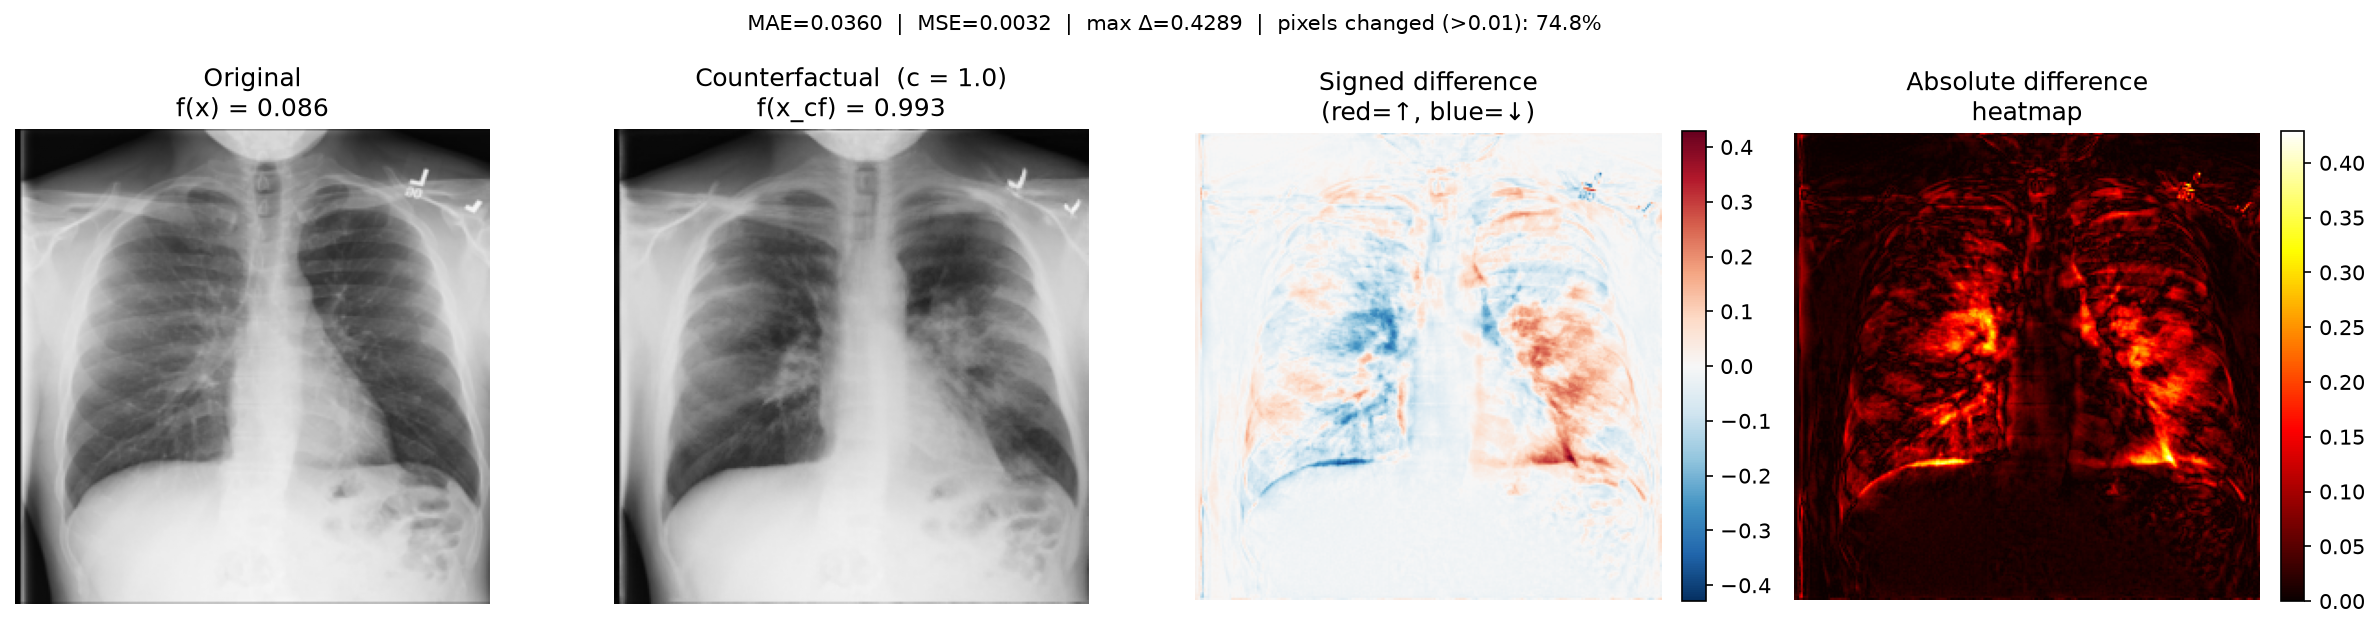
\includegraphics[width=\textwidth]{counterfactual_diff_n_to_p_ensemble.png}
  \caption[Ensemble-trained counterfactual: normal to pneumonia]{\textbf{Normal $\rightarrow$ pneumonia, ensemble-trained policy.}
  Left to right: original, counterfactual targeting $c=1$, signed pixel
  difference, and absolute-difference heatmap. Compare with
  Figure~\ref{fig:n2p}.}
  \label{fig:closing_n2p}
\end{figure}

\begin{figure}[h]
  \centering
  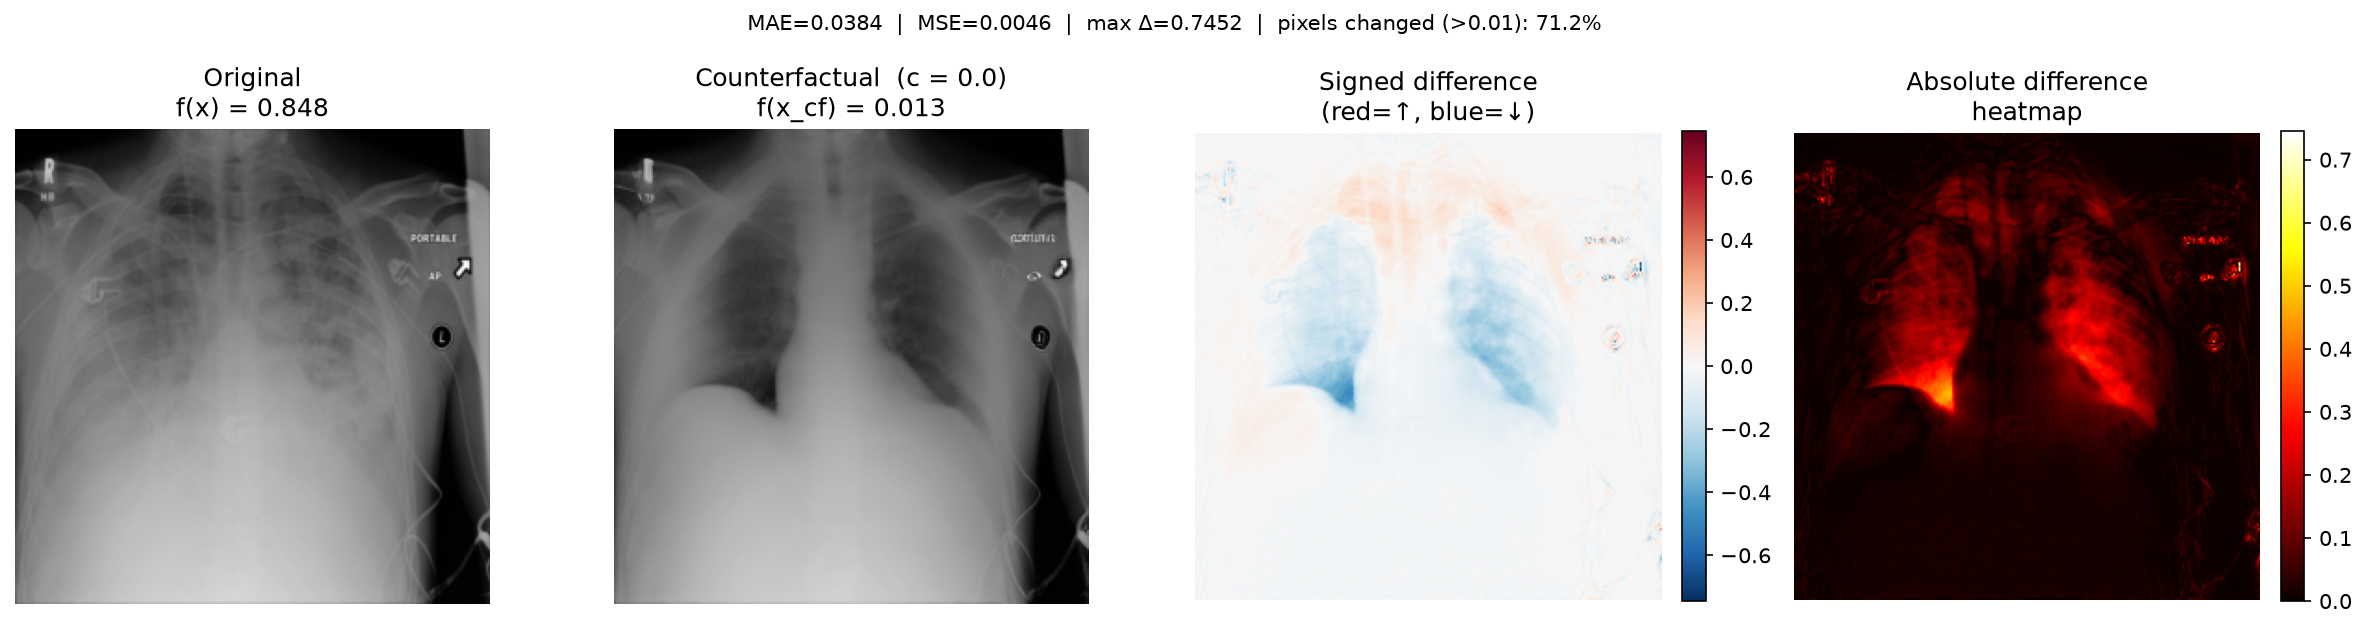
\includegraphics[width=\textwidth]{counterfactual_diff_p_to_n_ensemble.png}
  \caption[Ensemble-trained counterfactual: pneumonia to normal]{\textbf{Pneumonia $\rightarrow$ normal, ensemble-trained policy.}
  Same four-panel layout. Compare with Figure~\ref{fig:p2n}.}
  \label{fig:closing_p2n}
\end{figure}

Gross anatomical layout outside the lung field remains visibly intact in
both directions, consistent with the background lock holding under the
new guidance configuration exactly as it did under the old one --- the
change between the two policies is in \emph{what} guides the edit, not in
the structural guarantee that constrains where it can land.

\section{The Held-Out Transfer Result}
\label{sec:closing_transfer}

The held-out transfer procedure from Chapter~\ref{ch:integrity} was run
against both the new, ensemble-trained counterfactuals and the original,
single-classifier-trained ones, unchanged since Chapter~\ref{ch:results},
scored by the same three independent validators used throughout
Chapter~\ref{ch:integrity}: \texttt{nih}, \texttt{pc}, and
\texttt{mimic\_ch}. This set, not Table~\ref{tab:heldout}'s
\texttt{\{chex, nih\}}, is the correct comparison: \texttt{chex} is now a
guidance-ensemble member for the new policy, so scoring it as ``held out''
would let the new arm improve purely by losing a validator rather than by
editing more honestly --- exactly the mistake the denominator discipline
introduced in Section~\ref{sec:denominator_bug} exists to prevent.

\begin{table}[h]
\centering
\caption[Held-out transfer, before and after real ensemble training]{Held-out
transfer ratio ($\Delta_{\text{validator}}/\Delta_{\text{guidance}}$), single-
vs.\ ensemble-guided \emph{trained} policies, $n=200$ per group,
validators \texttt{\{nih, pc, mimic\_ch\}}.}
\label{tab:closing_transfer}
\begin{tabular}{@{}lrrrrrr@{}}
\toprule
& \multicolumn{2}{c}{\textbf{nih}} & \multicolumn{2}{c}{\textbf{pc}} & \multicolumn{2}{c}{\textbf{mimic\_ch}} \\
\cmidrule(lr){2-3}\cmidrule(lr){4-5}\cmidrule(lr){6-7}
\textbf{Policy} & \ntop{} & \pton{} & \ntop{} & \pton{} & \ntop{} & \pton{} \\
\midrule
Single-classifier (old) & $0.080$ & $0.100$ & $0.414$ & $0.224$ & $0.197$ & $0.112$ \\
Ensemble-guided (new)   & $0.046$ & $0.186$ & $0.462$ & $0.308$ & $0.337$ & $0.384$ \\
\bottomrule
\end{tabular}

\vspace{0.3em}
\begin{tabular}{@{}lrr@{}}
\toprule
\textbf{Policy} & \textbf{Mean \ntop{}} & \textbf{Mean \pton{}} \\
\midrule
Single-classifier (old) & $0.230$ & $0.146$ \\
Ensemble-guided (new)   & $\mathbf{0.282}$ & $\mathbf{0.293}$ \\
\bottomrule
\end{tabular}
\end{table}

\textbf{It mostly worked.} Mean transfer rose on both directions ---
\pton{} very nearly doubled ($0.146 \to 0.293$), matching what the
no-policy ensemble sweep (Table~\ref{tab:ensemble_sweep}) predicted, now
confirmed with an actually-trained policy rather than the fixed default
sampling schedule that sweep used. Two of the three validators, \texttt{pc}
and \texttt{mimic\_ch}, improved on both directions.

\textbf{It did not work uniformly.} \texttt{nih} --- the toughest and most
independent of the three validators, sharing no training data with any
guidance-ensemble member --- improved on \pton{} ($0.100 \to 0.186$) but
\emph{worsened} on \ntop{} ($0.080 \to 0.046$), remaining clearly in the
adversarial range on both counts. The honest reading is not ``the
adversarial gap is closed,'' but ``ensemble guidance measurably narrows it
against two of three independent classifiers, while the hardest one shows
no improvement in the direction that matters least favourably for this
claim.'' Section~\ref{sec:heldout}'s central warning --- that a system's
own validity number should not be trusted without an independent,
adversarially-chosen check --- applies with undiminished force to this
result too: \texttt{nih} was the check that did not confirm the story the
other two validators tell.

\section{The Trained-vs-Random Paired Significance Test}
\label{sec:closing_significance}

The second open item did not require new training: the paired per-image
test from Chapter~\ref{ch:integrity} was run against the existing
\texttt{trained} and \texttt{random} arms that produced
Table~\ref{tab:lhr_arms}'s control-arm row --- the same 183 images,
single-classifier-guided, that chapter left untested at the per-image
level.

\begin{table}[h]
\centering
\caption[Paired trained-vs-random significance test]{Paired per-image LHR
lift, trained vs.\ random, $n=183$ shared images (\pton{}).}
\label{tab:closing_significance}
\begin{tabular}{@{}lr@{}}
\toprule
Mean lift, trained & $2.293 \pm 0.780$ \\
Mean lift, random  & $2.204 \pm 0.772$ \\
Paired difference (95\% CI) & $+0.090$ $[+0.021,\ +0.160]$ \\
Paired $t$-test & $t=2.551$, $p=0.0116$ \\
Wilcoxon signed-rank & $p=0.0147$ \\
Cohen's $d$ (paired) & $0.189$ \\
Trained better on & $105/183$ images \\
\bottomrule
\end{tabular}
\end{table}

The gap survives: both the paired $t$-test and its non-parametric check
agree the trained policy edits closer to the radiologist's box than an
untrained one at the same action bounds and step budget, at $p<0.05$ by
either test. The right reading to close on, though, is the effect size
rather than the significance: a Cohen's $d$ of $0.189$ against a
between-image standard deviation of $0.78$ is a \emph{small} effect. Eight
hundred episodes of PPO bought a real, statistically detectable
improvement over an untrained policy with the same action bounds --- not a
large one.

\section{What This Closes, and What Is Still Open}

Table~\ref{tab:closing_summary} restates Section~\ref{sec:future}'s two
highest-priority items against what this chapter found.

\begin{table}[h]
\centering
\caption[Status of the two items this chapter addresses]{Future-work items
from Section~\ref{sec:future}, resolved.}
\label{tab:closing_summary}
\begin{tabular}{@{}p{0.55\textwidth}p{0.35\textwidth}@{}}
\toprule
\textbf{Item} & \textbf{Status} \\
\midrule
Complete the validation loop: re-run held-out validation against ensemble
guidance, trained (not just no-policy) &
Done (\S\ref{sec:closing_transfer}). Transfer improves on 2/3 validators
and both directions on average; \texttt{nih} \ntop{} does not improve. \\
\addlinespace
Resolve the trained-vs-random paired significance test &
Done (\S\ref{sec:closing_significance}). Significant, $p=0.012$, small
effect ($d=0.19$). \\
\bottomrule
\end{tabular}
\end{table}

\subsection{Is the \texttt{nih} Regression Real, or Noise?}
\label{sec:transfer_bootstrap}

The point estimates in Table~\ref{tab:closing_transfer} cannot answer that
by themselves --- a single run at $n=200$ per group. A percentile
bootstrap CI closes the gap: 10,000 resamples of the per-image
classifier-score deltas, resampling image indices jointly for the
guidance-classifier delta and the validator delta so the within-image
pairing is preserved (this is a ratio-of-means CI on \emph{one} policy's
shards, not a paired-difference CI across the two policies --- see the
caveat on pairing below).

\begin{table}[h]
\centering
\caption{Bootstrap 95\% CI on the nih transfer ratio, $n=200$ per
group, 10,000 resamples.}
\label{tab:transfer_bootstrap}
\begin{tabular}{@{}lrr@{}}
\toprule
\textbf{Policy} & \textbf{\ntop{} (point, 95\% CI)} & \textbf{\pton{} (point, 95\% CI)} \\
\midrule
Single-classifier (old) & $0.080$ $[0.048, 0.114]$ & $0.100$ $[0.076, 0.126]$ \\
Ensemble-guided (new)   & $0.046$ $[0.007, 0.084]$ & $0.186$ $[0.155, 0.216]$ \\
\bottomrule
\end{tabular}
\end{table}

\ntop{}: the two intervals overlap ($[0.048, 0.114]$ vs.\ $[0.007, 0.084]$),
so the apparent regression is \emph{not} statistically distinguishable from
noise at this sample size. Both intervals sit entirely below the $0.15$
adversarial threshold, so what the data does establish is that \ntop{}
stays confidently adversarial under \emph{both} policies --- not that
ensemble guidance made it worse. \pton{}: the intervals do not overlap
($[0.076, 0.126]$ vs.\ $[0.155, 0.216]$), so that improvement is real.

\textbf{Why not a joint difference-of-ratios bootstrap?} Because the two
policies' \texttt{Xn}/\texttt{Xp} groups are not the same images by index:
the classifier used to sort images into those groups changed between runs
(single-\texttt{rsna} $\to$ 2-member ensemble), and checking the shard
index sets directly shows they share only $\approx$70\% of \texttt{Xn} and
$\approx$24\% of \texttt{Xp}. A resample that treated the two arms as
paired by index would be synthesizing a pairing that does not exist in the
data, exactly the mistake Section~\ref{sec:denominator_bug} exists to
prevent for a different quantity. Reporting each policy's CI separately,
with non-overlap as the signal, is the honest version of this comparison.

\subsection{Diagnosing the Grad-CAM Degradation}
\label{sec:gradcam_diag}

Section~\ref{sec:arm_results} left one item explicitly unresolved: the
Grad-CAM spatial mask (\texttt{USE\_GRADCAM\_MASK}, ARM~2) measurably
\emph{lowered} lesion-targeting lift instead of raising it (cm0
$2.057 \to$ cm2 $1.534$, Table~\ref{tab:lhr_arms}) --- the opposite of its
design intent. A comment left in the training loop
(\file{factory/ppo.py}) speculated why: on synthetic probes, the
\texttt{rsna} ensemble member supposedly returned a degenerate Grad-CAM
far more often than \texttt{chex}, concentrated near predicted probability
$\approx 0.5$, attributed to Grad-CAM's all-negative-contribution edge
case rather than output saturation. That speculation had never been
tested against real data.

\texttt{check\_classifier\_localization.py} was extended to test it
directly: 150 images sampled across the \emph{full} probability range
(not just known-positives, which skew toward high pneumonia probability
and would under-represent the region the hypothesis is about), plus 150
known-positive boxed images for a lesion-overlap arm, scored through the
exact \texttt{ensemble\_grad\_cam} path
\texttt{compute\_gradcam\_latent\_mask} calls during PPO --- not a
reimplementation, the same code.

\begin{table}[h]
\centering
\caption{Grad-CAM degeneracy diagnostic, 263 member-image observations,
target layer \texttt{features} (the trained default).}
\label{tab:gradcam_diag}
\begin{tabular}{@{}lrl@{}}
\toprule
\textbf{Member} & \textbf{Degenerate} & \textbf{Where} \\
\midrule
\texttt{rsna} & $1/263$ ($0.4\%$) & negligible at every probability \\
\texttt{chex} & $66/263$ ($25.1\%$) & concentrated near $p \approx 0$
($64\%$ at $[0,0.1)$, falling to $0\%$ by $[0.7,0.9)$) \\
\bottomrule
\end{tabular}
\end{table}

\textbf{The hypothesis was backwards on every count.} It is \texttt{chex},
not \texttt{rsna}, that degenerates, at a materially higher rate ($25\%$
of episodes, not an occasional occurrence) than the earlier spot-check
suggested, and the degeneracy sits at \emph{low} probability, not near
$0.5$ --- which matches the \emph{original} explanation already on record
in \file{src/gradcam.py} (a saturated output zeroing the gradient) rather
than the newer all-negative-contribution hypothesis the training-loop
comment proposed.

This matters because of what happens when \texttt{chex} degenerates: the
averaged mask falls back toward \texttt{rsna} alone --- the
least-constrained, 2-head, easiest-to-fool ensemble member, the one the
whole ensemble-guidance defense exists to get away from
(Section~\ref{sec:heldout}) --- and CAM-lesion overlap drops with it. Mean
lift against real radiologist boxes was $2.052$ ($n=127$) on clean
episodes versus $1.347$ ($n=23$) on partially-degenerate ones. A quarter
of episodes losing a third of their lesion-targeting signal is a
plausible, now-quantified contributor to cm2's regression below even the
no-countermeasure baseline.

\textbf{The obvious fix does not work.} \file{config.py}'s own comment
suggested stepping down to a finer target layer
(\texttt{features.denseblock3}, $14\times14$ vs.\ the default $7\times7$)
if the mask looked too coarse. Repeating the same diagnostic with that
override does eliminate the degeneracy almost entirely (\texttt{chex}
$0\%$, \texttt{rsna} $0.4\%$) --- but at a cost that makes it worse, not
better, as a remedy: baseline CAM-lesion lift on clean episodes \emph{falls}
to $1.196$ ($n=149$), barely above the $1.0$ chance floor. The finer
layer's own localisation is markedly worse even when nothing degenerates,
so trading degeneracy for resolution is not a net improvement.

Read honestly, the Grad-CAM mask has two independent problems, not one:
it is partially unreliable (a real, now-quantified degeneracy rate at
roughly a quarter of episodes under the trained configuration), and, even
at its best, only loosely aligned with the true lesion (a $\sim2\times$
lift is a real signal, not chance, but far from the tight localisation the
mask's design assumes). The one remedy already on record for either
problem trades the first for a worse version of the second.

\subsection{A Trained 3-Model Ensemble}
\label{sec:ensemble3}

Table~\ref{tab:ensemble_sweep}'s 3-member ensemble
(\texttt{[rsna, chex, mimic\_nb]}) was only ever tested through the cheap
no-policy path in Chapter~\ref{ch:integrity} --- no PPO policy had
actually been trained under it. Both directions were retrained from
scratch: 800 episodes each, fresh state confirmed by the training log
(no ``resuming'' message, the resume-trap check from
Section~\ref{sec:closing} repeated before submitting), stored under a
dedicated checkpoint directory (\file{checkpoints\_ens3/}) so the
committed 2-model policies were never at risk. Everything else was held
at the committed default --- no Grad-CAM mask, no sparsity reward --- to
isolate the ensemble-size change alone, matching this project's ARM1/
ARM2/ARM3 convention. \texttt{mimic\_nb} shares its MIMIC-CXR corpus with
the \texttt{mimic\_ch} validator, so held-out transfer here is scored on
the reduced, leak-free set \texttt{\{nih, pc\}} only, matching the
no-policy sweep's own convention (Section~\ref{sec:denominator_bug}) ---
\texttt{config.py} and \texttt{domains/rsna\_pneumonia.py} were reverted
to the committed default immediately after this experiment's evaluation
completed.

\begin{table}[h]
\centering
\caption{Held-out transfer ratio, 2- vs.\ 3-model ensemble-guided
\emph{trained} policies, $n=200$ per group, leak-free validators
\texttt{\{nih, pc\}}, with bootstrap 95\% CIs.}
\label{tab:ensemble3_transfer}
\begin{tabular}{@{}lrr@{}}
\toprule
\textbf{Validator / direction} & \textbf{2-model} & \textbf{3-model} \\
\midrule
nih \ntop{} & $0.046$ $[0.007,0.084]$ & $0.076$ $[0.033,0.119]$ \\
nih \pton{} & $0.186$ $[0.155,0.216]$ & $0.251$ $[0.167,0.337]$ \\
pc \ntop{}  & $0.462$ $[0.433,0.491]$ & $\mathbf{0.623}$ $[0.597,0.648]$ \\
pc \pton{}  & $0.308$ $[0.282,0.336]$ & $0.301$ $[0.218,0.388]$ \\
\midrule
Mean \ntop{} & $0.254$ & $\mathbf{0.350}$ \\
Mean \pton{} & $0.247$ & $\mathbf{0.276}$ \\
\bottomrule
\end{tabular}
\end{table}

\textbf{\texttt{pc} improved for real.} \ntop{} moved from $0.462$ to
$0.623$ --- the CIs, $[0.433,0.491]$ vs.\ $[0.597,0.648]$, do not
overlap, and the verdict itself flips from \texttt{arm\_transfer.py}'s
``partial'' to ``TRANSFERS''. \texttt{pc} \pton{} stayed flat
($0.308 \to 0.301$, heavily overlapping CIs).

\textbf{\texttt{nih} moved the right way, but not past noise.} Both
directions improved in point-estimate terms (\ntop{}
$0.046 \to 0.076$; \pton{} $0.186 \to 0.251$), but the CIs overlap on
both ($[0.007,0.084]$ vs.\ $[0.033,0.119]$; $[0.155,0.216]$ vs.\
$[0.167,0.337]$) --- the same bootstrap machinery from
Section~\ref{sec:transfer_bootstrap} says this movement is not
distinguishable from noise at $n=200$. Both policies stay confidently
below the $0.15$ adversarial threshold on \ntop{} regardless.

\textbf{Guidance-side metrics kept moving the expected direction.} CV
fell further, to a mean of $0.624$ (\ntop{} $0.685$, \pton{} $0.563$) ---
consistent with the pattern already established across every ensemble
size tried: a harder joint consensus criterion, not a weaker policy. LHR
lift was $2.492$, against the 2-model arm's $2.673$ --- but on a much
smaller annotated overlap ($n=27$ vs.\ $148$ pairs), since the harder
consensus criterion shrinks the classifier-negative-but-clinically-positive
group LHR depends on. That is a sample-size caveat worth stating plainly,
not a confident regression claim on top of everything else this
experiment measured.

\textbf{Read honestly:} a real, trained 3-model ensemble buys a genuine,
statistically confirmed improvement on \texttt{pc}, and moves \texttt{nih}
in the right direction on both counts without closing the adversarial gap
in a way this sample size can confirm. It does not fully resolve the
\texttt{nih} regression this chapter opened with, but nothing in this
experiment suggests the larger ensemble makes anything worse.

\subsection{A Trained Sparsity-Reward Arm}
\label{sec:sparsity_arm}

Edit concentration --- the share of total $|\Delta|$ carried by the top
5\% of pixels --- has stayed diffuse (0.25--0.32 against a 0.05 uniform
baseline) in every arm measured so far, never approaching the
$\sim$0.5 that would indicate a focal, lesion-shaped edit.
\texttt{USE\_SPARSITY\_REWARD} was built in Chapter~\ref{ch:tasks}
specifically to address this, but has sat disabled since 2026-08-07
(``REVERTED, was ARM 3''), which left its annealing ramp
(\texttt{USE\_SPARSITY\_ANNEALING}) inert --- the term has never actually
fired in any result reported so far, including every diffuse-edit number
quoted above.

It was re-enabled for an isolated retrain: only \texttt{USE\_SPARSITY\_REWARD}
flips relative to the committed default (2-model ensemble, no Grad-CAM
mask), so \texttt{SPARSITY\_OUTSIDE\_CAM\_ONLY} degrades to a plain,
unweighted L1 penalty on total edit magnitude --- a deliberate, flagged
choice (\texttt{factory/ppo.py} now prints a NOTE for this exact
situation), not an oversight. Both directions were retrained from
scratch, 800 episodes each, fresh state confirmed by the training log,
which also confirms $\lambda_{\text{sparsity}}$ genuinely ramped to its
target of $2.0$ this time.

\begin{table}[h]
\centering
\caption{Committed default vs.\ trained sparsity-reward arm.}
\label{tab:sparsity_results}
\begin{tabular}{@{}lrr@{}}
\toprule
\textbf{Metric} & \textbf{Default} & \textbf{+ sparsity reward} \\
\midrule
EditConcentration \ntop{} & $0.253$ & $0.264$ \\
EditConcentration \pton{} & $0.318$ & $0.299$ \\
CV mean & $0.838$ & $0.830$ \\
LHR lift (\pton{}) & $2.673$ & $2.398$ \\
Mean transfer \ntop{} & $0.282$ & $0.311$ \\
Mean transfer \pton{} & $0.293$ & $0.212$ \\
\bottomrule
\end{tabular}
\end{table}

\textbf{It did not achieve its own goal.} Edit concentration moved by
less than $0.02$ in either direction, and the fraction of pixels touched
stayed within $0.01$ of the default ($0.650\to0.661$, $0.633\to0.632$)
--- nowhere near the $\sim$0.5 focal threshold, despite the term now
being genuinely active rather than inert.

\textbf{It made lesion targeting measurably worse.} A paired test
(the same machinery from Section~\ref{sec:closing_significance}) on the
$148$ annotated images both arms share gives a lift gap of $+0.275$
favouring the arm \emph{without} the sparsity reward (95\% CI
$[+0.188, +0.363]$), $t=6.229$, $p=4.7\times10^{-9}$, Wilcoxon
$p=1.2\times10^{-8}$, Cohen's $d=0.512$ --- a \emph{medium} effect,
markedly larger than the trained-vs-random gap found in
Section~\ref{sec:closing_significance} ($d=0.189$). The default arm was
better on $104/148$ images.

\textbf{It made held-out transfer worse in the \pton{} direction.} Mean
\pton{} transfer fell from $0.293$ to $0.212$, driven by real,
non-overlapping-CI drops on two of three validators: \texttt{pc}
($0.308\to0.216$, CIs $[0.282,0.336]$ vs.\ $[0.192,0.242]$) and
\texttt{mimic\_ch} ($0.384\to0.252$, CIs $[0.343,0.422]$ vs.\
$[0.212,0.292]$). \ntop{} transfer moved slightly up on average
($+0.029$) but no single validator's CI shift clears overlap.

Read plainly: enabling the sparsity reward for real, rather than leaving
its annealing ramp inert, does not concentrate edits --- its designed
purpose --- and instead costs both lesion-targeting lift and \pton{}
transfer, each by a real, measured margin, not noise. A plain
(non-CAM-weighted) L1 penalty discourages edit mass uniformly rather than
specifically off-target mass, which is a plausible explanation for why it
competes with precise editing without succeeding at its own goal: whether
a working spatial mask --- unresolved by this chapter's own Grad-CAM
diagnosis above --- would change that outcome remains untested.

\subsection{A Trained Grad-CAM-Fix Arm}
\label{sec:gradcam_fix_arm}

Section~\ref{sec:gradcam_diag}'s diagnosis was deliberately an
\emph{offline} probe --- Grad-CAM computed on real images, scored against
ground-truth lesion boxes, with no PPO policy or generated counterfactual
anywhere in the loop. It found \texttt{features.denseblock3} nearly
eliminates ensemble degeneracy but at a real cost to the CAM's own
baseline lesion overlap. That is suggestive evidence the layer swap is
not a fix, but it falls short of the standard every other claim in this
chapter is held to: a real policy, trained and fully evaluated. So one
was trained: \texttt{USE\_GRADCAM\_MASK=True},
\texttt{GRADCAM\_TARGET\_LAYER=features.denseblock3}, everything else at
the committed default (2-model ensemble, no sparsity reward), both
directions from scratch. The first submission for \ntop{} exhausted its
22h wall-clock budget at 49\% (392/800 episodes, 42.5 minutes per PPO
update at this resolution --- markedly slower than any other arm in this
project) and paused cleanly; a second submission resumed from checkpoint
and completed it. \pton{} finished in one submission.

\begin{table}[h]
\centering
\caption{Committed default vs.\ trained Grad-CAM-fix arm.}
\label{tab:gradcam_fix_results}
\begin{tabular}{@{}lrr@{}}
\toprule
\textbf{Metric} & \textbf{Default} & \textbf{+ Grad-CAM fix} \\
\midrule
CV mean & $0.838$ & $\mathbf{0.017}$ \\
LHR lift (\pton{}) & $2.673$ & $1.636$ \\
Mean transfer \ntop{} & $0.282$ & $0.161$ \\
Mean transfer \pton{} & $0.293$ & $0.103$ \\
\bottomrule
\end{tabular}
\end{table}

\textbf{This is unambiguous, not another ``partial'' result.} CV
collapsed from a mean of $0.838$ to $0.017$ --- the policy essentially
stopped succeeding at the base task (flipping the guidance ensemble)
under this constrained action space; a finer, less-confident CAM region
does not merely localise worse, it makes the classifier-flip itself hard
to learn within the same reward budget and step count tuned for the
unconstrained case. The paired LHR test on the $148$ shared annotated
images gives a lift gap of $+1.037$ favouring the arm \emph{without} the
Grad-CAM constraint (95\% CI $[+0.900, +1.178]$), $t=14.660$,
$p=1.5\times10^{-30}$, Wilcoxon $p=1.7\times10^{-22}$, Cohen's
$d=1.205$ --- the largest paired effect size measured anywhere in this
project, well past the sparsity arm's $d=0.512$ and an order of magnitude
past the original trained-vs-random gap's $d=0.189$. The default arm was
better on $141$ of $148$ images. Held-out transfer fell across all three
validators, with \texttt{nih} and \texttt{mimic\_ch} moving into or
staying in \texttt{arm\_transfer.py}'s \texttt{ADVERSARIAL} band on both
directions.

Read plainly: this is not a fix, and now that is confirmed rather than
merely diagnosed. Trading a manageable degeneracy problem for a
finer-but-less-confident CAM does not net out positive --- it makes
learning the base task substantially harder, and every metric downstream
of that task degrades with it. \texttt{USE\_GRADCAM\_MASK} stays off in
the committed configuration; the config edit was reverted immediately
after this experiment's evaluation completed.

Six items across this chapter and the last now have numbers rather than
open questions attached to them: the two \emph{Table~\ref{tab:closing_summary}}
originally addressed, why the Grad-CAM constraint hurts (diagnosed),
whether a larger trained ensemble would help \texttt{nih} (partial,
honest: yes for \texttt{pc}, not conclusively for \texttt{nih}), whether
the sparsity reward would concentrate edits (no, and it costs targeting
accuracy), and whether the one Grad-CAM remedy already on record actually
fixes the constraint once a real policy is trained under it (no ---
confirmed, not just suspected). None is closed in the sense of settling
the project's central claim. Ensemble guidance is confirmed, with a
trained policy and the correct leak-free validator set, to be a real
partial countermeasure --- and \texttt{nih}'s \ntop{} result is
confirmation that ``partial'' is the accurate word, not a hedge. What
remains is whether \emph{any} Grad-CAM mask can help rather than hurt,
whether \texttt{nih} specifically would need a larger annotated sample or
a different guidance composition to move past noise, and whether edit
diffuseness is fixable at all within this gradient-guidance approach. The
previous single-classifier policies and their counterfactuals were
archived, not overwritten, specifically so that this comparison remains
reproducible.

\section{Comparing All Five Arms}
\label{sec:five_arm_comparison}

Five checkpoint directories now hold a fully trained, fully evaluated
policy under this chapter's protocol: the archived single-classifier
baseline (\file{checkpoints/archive\_pre\_ensemble\_default\_20260812/}),
the committed 2-model-ensemble default (\file{checkpoints/}), and the
three isolated retrains above ---
\file{checkpoints\_ens3/}, \file{checkpoints\_sparsity/},
\file{checkpoints\_gradcam\_fix/}. Every number below comes from that same
800-episode-per-direction, 200-image-per-group pipeline --- none is a
no-policy countermeasure sweep or an offline proxy, and every ``confirmed''
claim is backed by a paired significance test or a bootstrap CI run
specifically for this comparison, not a point estimate read off a table.

\begin{figure}[h]
\centering
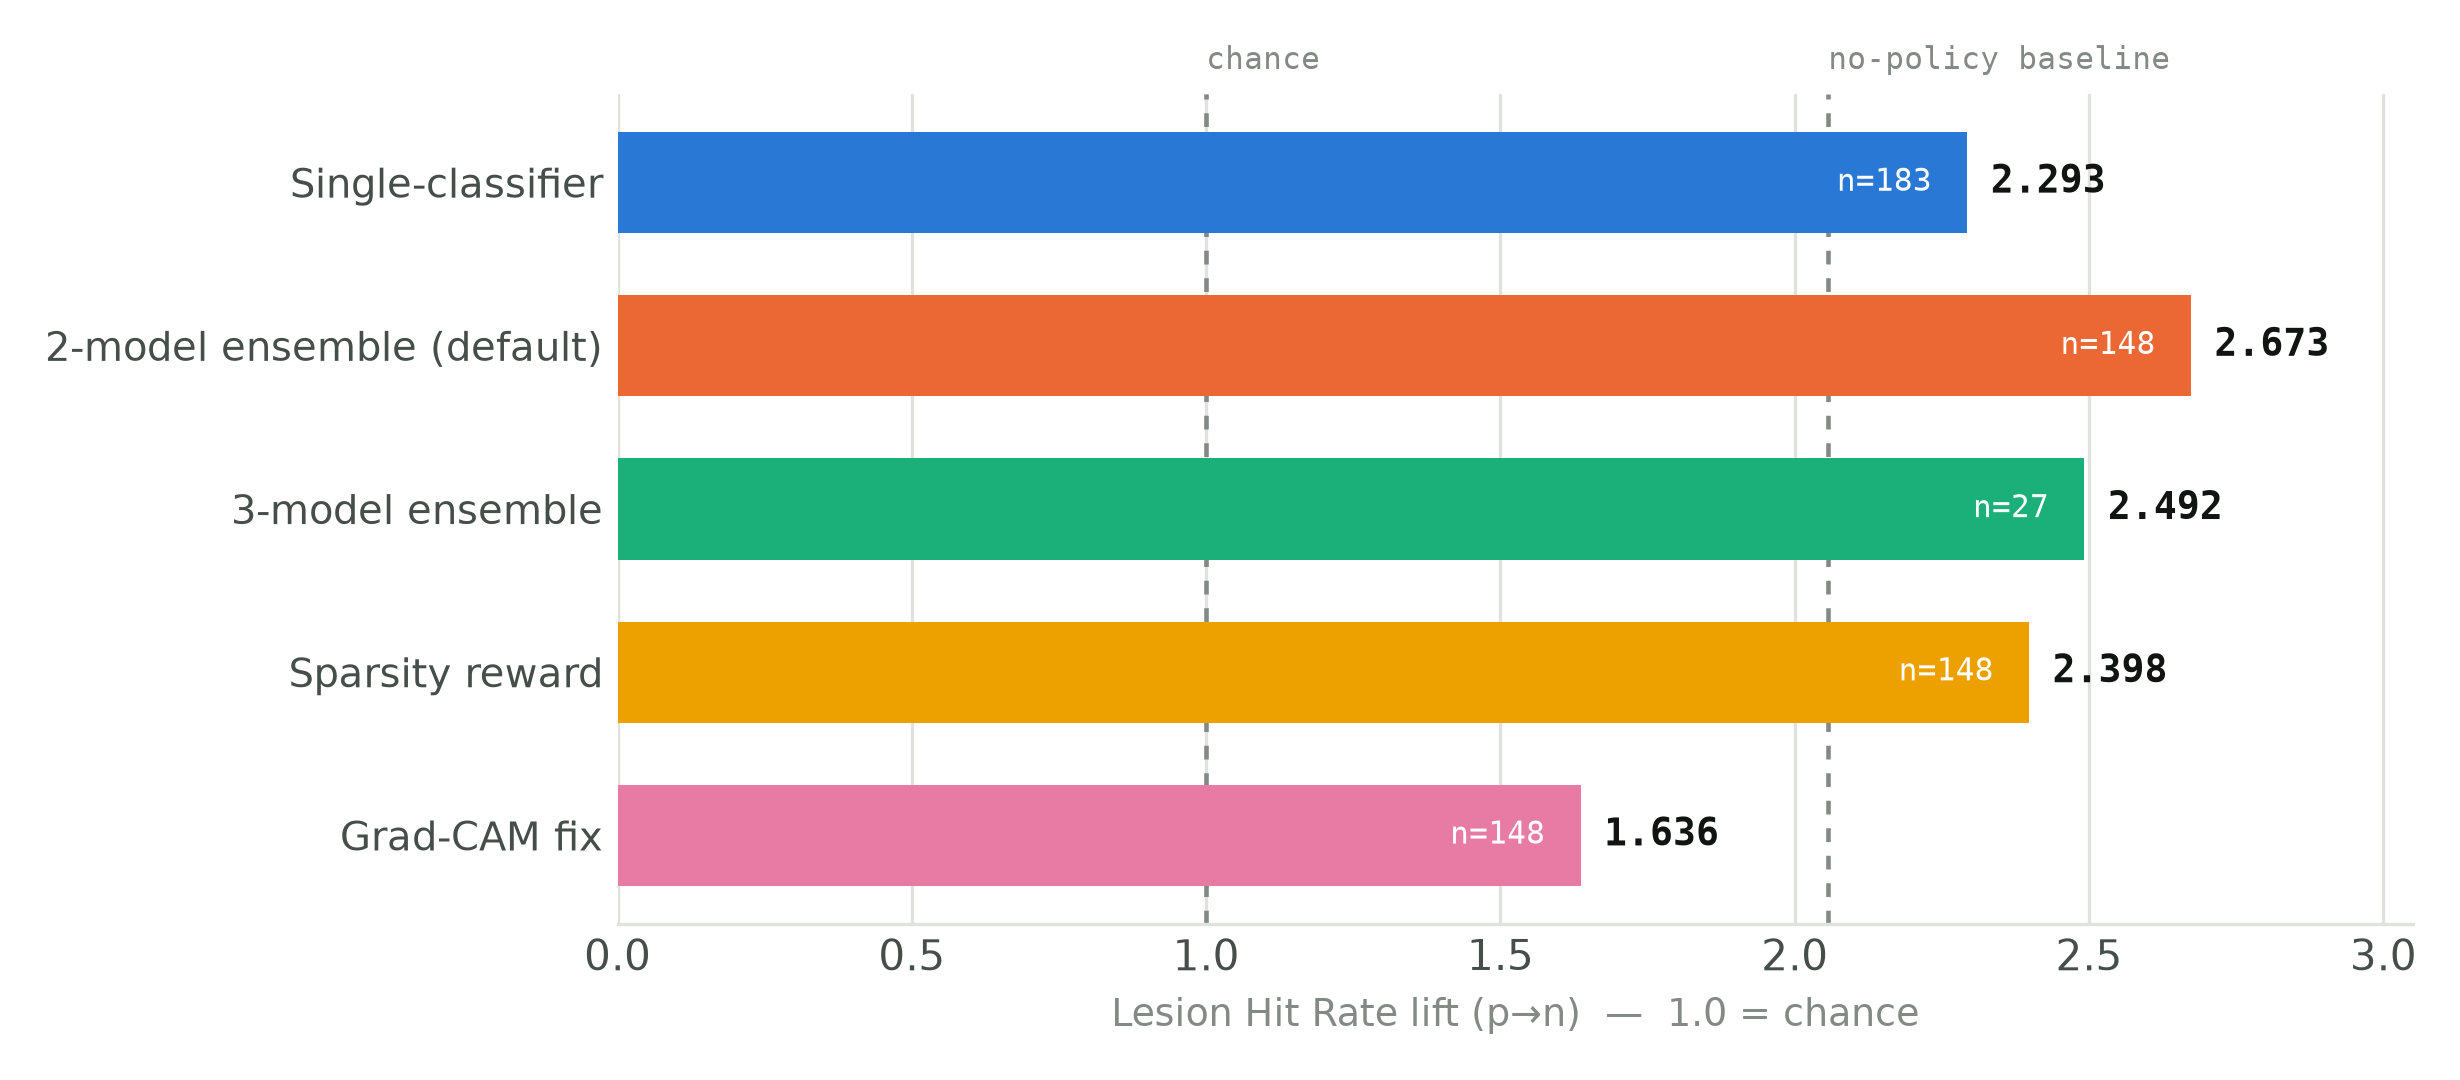
\includegraphics[width=\textwidth]{chart_lhr_lift.png}
\caption{Lesion Hit Rate lift (\pton{}) across all five trained arms.
Dashed lines mark chance ($1.0$) and the no-policy label-protocol baseline
($2.057$, Table~\ref{tab:lhr_arms}'s cm0 row).}
\label{fig:five_arm_lhr}
\end{figure}

\begin{figure}[h]
\centering
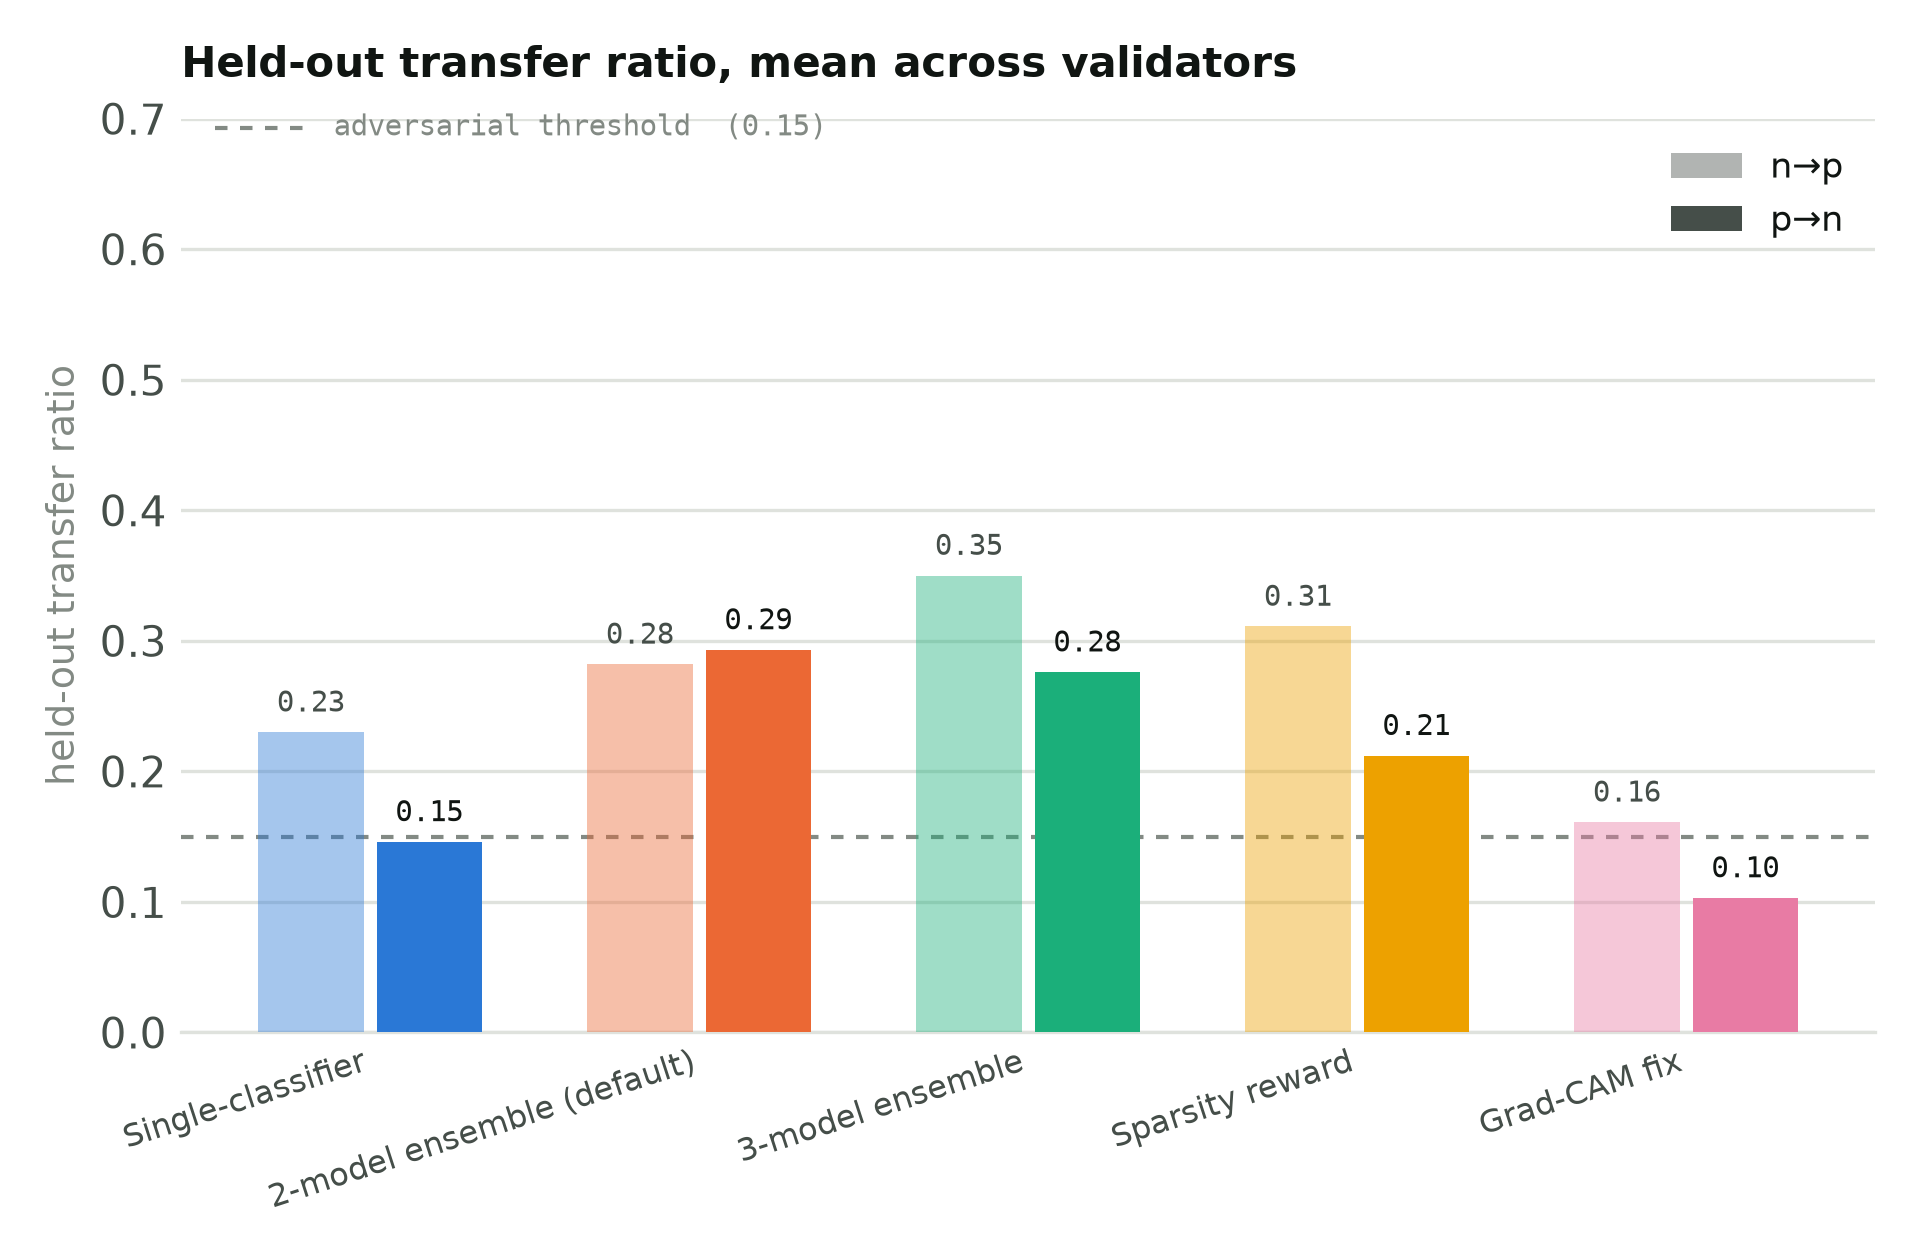
\includegraphics[width=0.49\textwidth]{chart_transfer_ratio.png}
\hfill
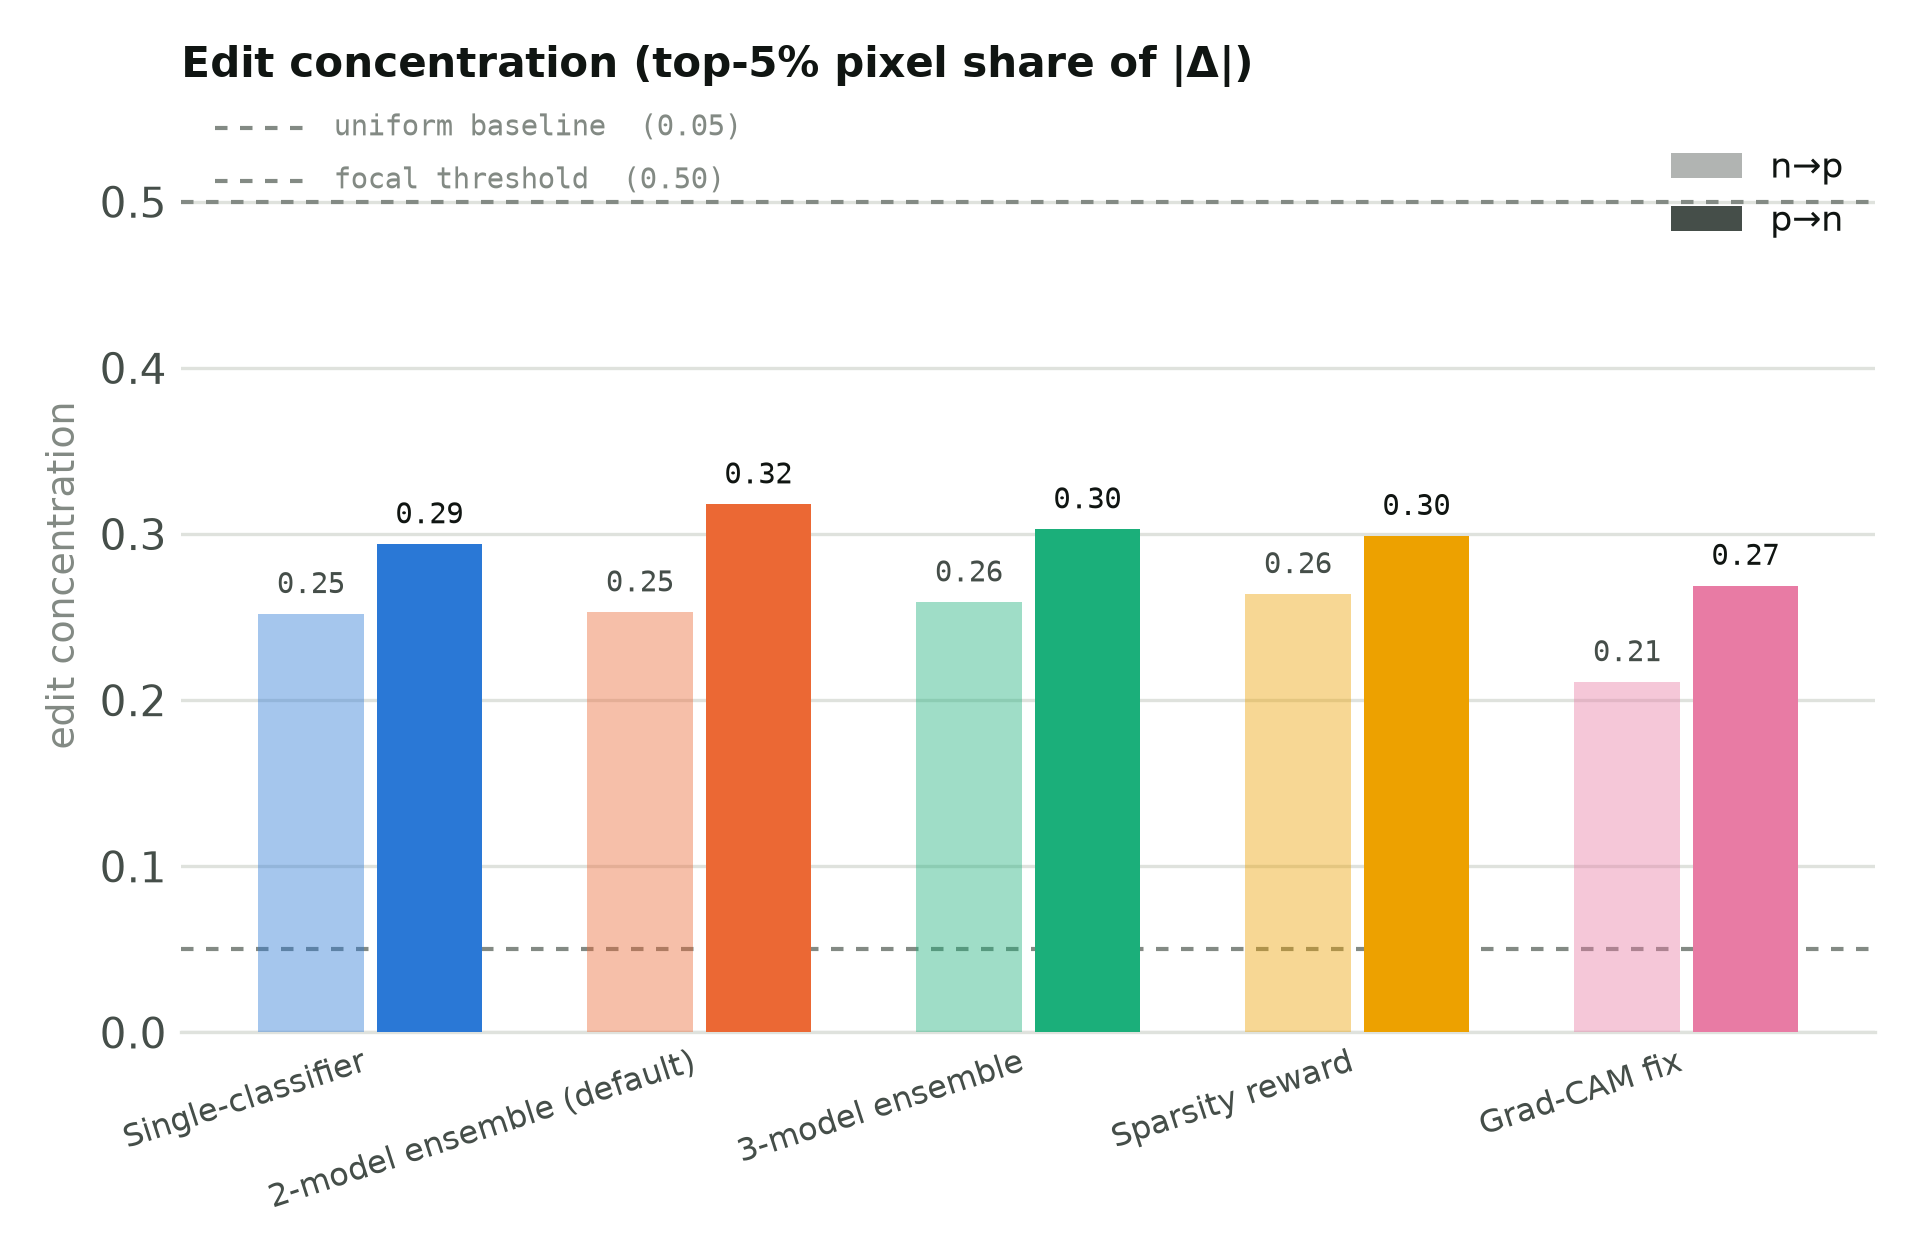
\includegraphics[width=0.49\textwidth]{chart_edit_concentration.png}
\caption{Held-out transfer ratio (left) and edit concentration (right)
across all five arms. The 3-model ensemble's transfer figure is scored on
the reduced validator set \texttt{\{nih, pc\}} only (Section~\ref{sec:ensemble3})
and is not directly comparable to the other four arms' 3-validator mean.}
\label{fig:five_arm_transfer_concentration}
\end{figure}

\textbf{Reading the three figures against the paired tests run for each
pair, throughout this chapter:} the single-classifier $\to$
2-model-ensemble step is a confirmed real gain in \pton{} LHR lift
($d=0.482$, $p=7.1\times10^{-5}$, $n=76$ shared annotated images --- a
smaller paired sample than the other comparisons, since the two arms'
Xn/Xp groups only partially overlap once the group-selection classifier
changes). The 2-model $\to$ 3-model-ensemble step is \emph{not}
statistically resolved on LHR: only 12 images are shared between those two
arms' annotated sets, giving a paired CI of $[-0.298, +0.482]$ that
crosses zero --- too wide to read anything into, even though \texttt{pc}
transfer improved for real on its own bootstrap CI (Section~\ref{sec:ensemble3}).
Both the sparsity-reward and Grad-CAM-fix retrains are confirmed worse
than the default: $d=0.512$ ($p=4.7\times10^{-9}$) for sparsity,
$d=1.205$ ($p=1.5\times10^{-30}$) for the Grad-CAM fix --- the largest
paired effect size measured anywhere in this project, by a wide margin.

\textbf{No arm moved edit concentration.} Every bar in the right-hand
panel of Figure~\ref{fig:five_arm_transfer_concentration} sits in the same
$0.21$--$0.32$ band regardless of what changed underneath it --- ensemble
size, a sparsity penalty genuinely turned on, or a Grad-CAM constraint
that cratered every other metric. Across five independently trained
policies and every countermeasure this project tried, edit diffuseness
never moved appreciably toward the $\sim$0.5 threshold that would indicate
a focal, lesion-shaped edit. That consistency is itself a finding: this
looks less like a tuning problem specific to any one arm and more like a
property of gradient-guided diffusion editing on this generator, which
Section~\ref{sec:sparsity_arm}'s negative result is the closest this
project comes to testing directly.
